\chapter{Word2Vec}

El modelo \textit{word2vec} es una técnica para el procesamiento del lenguaje natural publicada en 2013 (\cite{word2vec:1}, \cite{word2vec:2}).
El algoritmo usa un modelo con una red neuronal para aprender asociaciones entre las palabras de un conjunto de texto. Una vez que el modelo ha
sido entrenado, es posible detectar sinónimos de palabras o incluso sugerir palabras en oraciones incompletas.

Como su nombre indica, \textit{word2vec} representa cada palabra mediante un vector. Estos vectores se escogen de forma que palabras semánticamente similares
estén relativamente cerca entre ellas. Para medir esta cercanía, se usa la similitud coseno:

\begin{definition}
  Dados dos vectores $a,b\in\mathbb{R}$, $n\in\mathbb{N}$, se define la similitud coseno como:
  \[
    S_c(a,b)=\cos\theta = \frac{a\cdot b}{\norm{a}\norm{b}} \in [-1, 1]
  \]
donde $\theta\in[-\pi,\pi]$ es el ángulo entre los vectores $a$ y $b$.
\end{definition}

Es importante notar que la similitud coseno no es una función de medida, ya que no cumple la desigualdad de Schwarz (o desigualdad triangular). El resultado
de esta función indica el nivel de similitud semántica entre las palabras representadas por esos vectores.

A continuación, se presenta cómo se van a obtener esos vectores, y posteriormente, cómo tratar esos vectores para obtener información sobre las palabras. Para
ello, se presentan dos variantes del modelo.

\section{Coninuous Bad-of-Word Model}

Primero se va a desarrollar el modelo \textit{bolsa de palabras continuas} (o CBOW, por sus siglas en inglés) considerando que el contexto está formado por una única palabra.
Esto será útil para establecer la notación para el resto del trabajo. Que haya una única palabra por contexto implica que el modelo precidirá también una única palabra objetivo.
Por lo tanto, se está presentando un modelo \textit{bigram} (es decir, que usa dos palabras).

\begin{figure}[H]
  \centering
  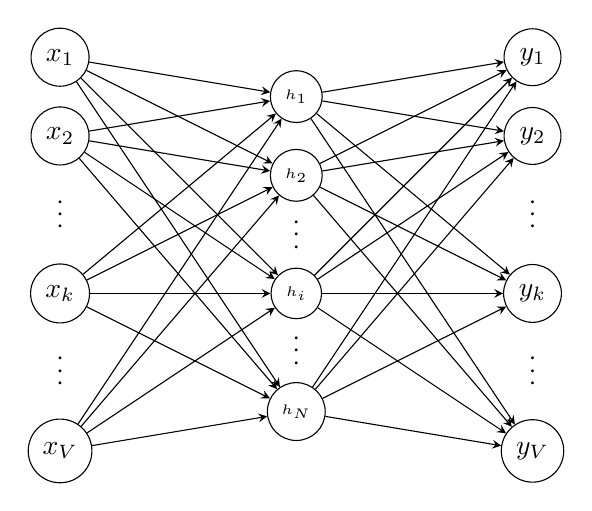
\begin{tikzpicture}[
          roundnode/.style={circle, draw=black, minimum size=4mm},
      ]

      \node[roundnode]   at (1,4)   (inputV)  {$x_V$};
      \node[roundnode]   at (1,6)   (inputK)  {$x_k$};
      \node[roundnode]   at (1,8)   (input2)  {$x_2$};
      \node[roundnode]   at (1,9)   (input1)  {$x_1$};

      \path (input2) -- (inputK) node [black, midway, sloped] {$\dots$};
      \path (inputK) -- (inputV) node [black, midway, sloped] {$\dots$};

      \node[roundnode]   at (4,4.5)   (hiddenN)  {\tiny $h_N$};
      \node[roundnode]   at (4,6)     (hiddenI)  {\tiny $h_i$};
      \node[roundnode]   at (4,7.5)   (hidden2)  {\tiny $h_2$};
      \node[roundnode]   at (4,8.5)   (hidden1)  {\tiny $h_1$};

      \path (hidden2) -- (hiddenI) node [black, midway, sloped] {$\dots$};
      \path (hiddenI) -- (hiddenN) node [black, midway, sloped] {$\dots$};

      \draw[-stealth] (input1) -- (hidden1);
      \draw[-stealth] (input1) -- (hidden2);
      \draw[-stealth] (input1) -- (hiddenI);
      \draw[-stealth] (input1) -- (hiddenN);
      \draw[-stealth] (input2) -- (hidden1);
      \draw[-stealth] (input2) -- (hidden2);
      \draw[-stealth] (input2) -- (hiddenI);
      \draw[-stealth] (input2) -- (hiddenN);
      \draw[-stealth] (inputK) -- (hidden1);
      \draw[-stealth] (inputK) -- (hidden2);
      \draw[-stealth] (inputK) -- (hiddenI);
      \draw[-stealth] (inputK) -- (hiddenN);
      \draw[-stealth] (inputV) -- (hidden1);
      \draw[-stealth] (inputV) -- (hidden2);
      \draw[-stealth] (inputV) -- (hiddenI);
      \draw[-stealth] (inputV) -- (hiddenN);


      \node[roundnode]   at (7,4)   (outputV)  {$y_V$};
      \node[roundnode]   at (7,6)   (outputI)  {$y_k$};
      \node[roundnode]   at (7,8)   (output2)  {$y_2$};
      \node[roundnode]   at (7,9)   (output1)  {$y_1$};

      \path (output2) -- (outputI) node [black, midway, sloped] {$\dots$};
      \path (outputI) -- (outputV) node [black, midway, sloped] {$\dots$};

      \draw[-stealth] (hidden1) -- (output1);
      \draw[-stealth] (hidden1) -- (output2);
      \draw[-stealth] (hidden1) -- (outputI);
      \draw[-stealth] (hidden1) -- (outputV);
      \draw[-stealth] (hidden2) -- (output1);
      \draw[-stealth] (hidden2) -- (output2);
      \draw[-stealth] (hidden2) -- (outputI);
      \draw[-stealth] (hidden2) -- (outputV);
      \draw[-stealth] (hiddenI) -- (output1);
      \draw[-stealth] (hiddenI) -- (output2);
      \draw[-stealth] (hiddenI) -- (outputI);
      \draw[-stealth] (hiddenI) -- (outputV);
      \draw[-stealth] (hiddenN) -- (output1);
      \draw[-stealth] (hiddenN) -- (output2);
      \draw[-stealth] (hiddenN) -- (outputI);
      \draw[-stealth] (hiddenN) -- (outputV);

  \end{tikzpicture}
  \caption{CBOW con 1 palabra por contexto}
  \label{redneuronal:3}
\end{figure}

En la figura \ref{redneuronal:3}, se muestra la versión simplificada de la red neuronal, donde el tamaño del vocabulario es $V\in\mathbb{N}$ y el tamaño de la capa escondida es $N\in\mathbb{N}$.
Las unidades entre capas adyacentes están conectadas totalmente a todas las unidades de la otra capa y viceversa. Como input de la red se usa un \textit{one-hot encoded vector},
que simplemente es un vector de tamaño $V$ donde cada posición representa una palabra. Es decir, si arbitrariamente, se deduce que la palabra 'coche` se va a representar en la $k-$ésima
posición, entonces el vector $(0, \dots, 1, \dots, 0)$ con un 1 en la $k-$ésima posición, sería la representación de la palabra coche.

Los pesos entra la capa de entrada y la de salida pueden ser representados por una matriz $W\in\mathbb{R}^{V\times N}$, donde cada fila de $W$ es la representación
vectorial $N-$dimensional de la palabra $w$ asociada en la capa de entrada. Las filas de esta matriz son la represención vectorial $N$-dimensional, $v_{w_I}$ (donde $I\in\{1, \ldots, V\}$),
de la palabra $w$ de entrada (representada por $x$).

Dado entonces un contexto con una única palabra, $w_I$, se tiene su representación como vector de entrada $x\in\mathbb{R}^V$, de forma que $x_k=1$ con $x_{k'}=0$ si $k'\neq k$. A partir de
$W$ y $x$, se puede obtener el vector $N$-dimensional de la capa intermedia, de la siguiente forma:
\[
  h=W^Tx=W^T_{k, \cdot}=v^T_{w_I}
\]
donde es importante resaltar que esta operación no es más que copiar la fila $k$-ésima de $W$ en $h$. Esa fila fue denotada en el párrafo anterior por $v_{w_I}$.
Esto significa que la función de activación de la capa escondida es simplemente linear, es decir, pasa directamente la suma ponderada de sus inputs a la siguiente capa.

De forma similar, se puede operar de la capa escondida a la capa de salida, donde se tiene una matriz de pesos diferente, $W'\in\mathbb{R}^{N\times V}$. En esta matriz, la representación
de cada palabra viene dada por cada una de sus columnas, es decir, la representación de la palabra $w_j$ en $W'$, es la columna $j$-ésima de $W'$ y es representada por $v'_{v_{w_j}}$. Con
esta notación, se puede calcular ahora un escalar (antes se ha calculado un vector) $u_j$ para cada una de las palabras del vocabulario:
\[
u_j = v_{w_j}^{'T}h
\]
Finalmente, se puede usar \textit{softmax}, un modelo de clasificación lineal logarítmico, para obtener una distribución de las palabras (que es una distribución multinomial):
\[
p(w_j|w_I) = \frac{\exp(u_j)}{\sum_{j'=1}^V\exp(u_{j'})} =: y_j
\]
donde $y_j$ es el valor de la $j$-ésima neurona de la capa de salida. Una vez se tiene esta expresión, se pueden sustituir los valores de $u_j$ y $u_j'$ por los obtenidos
en párrafos anteriors, llegando a la siguiente fórmula:
\[
p(w_j|w_I) = \frac{\exp(w^{'T}_{w_j}v_{w_I})}{\sum_{j'=1}^V\exp(v^{'T}_{w_{j'}}v_{w_I})}
\]
Como clarificación, es importante recordar que $v_w$ y $v'_w$, son representaciones distintas de la palabra $w$:
\begin{itemize}
  \item $v_w$ proviene de las filas de la matriz $W$. Normalmente es denominado el vector de entrada.
  \item $v'_w$ proviene de las columnas de la matriz $W'$. Normalmente es denominado el vector de salida.
\end{itemize}